% Seeded from ../notebooks/lesson_38.ipynb; source notebook is unchanged.
% Focus: ../pages/lesson_38.md (macro objective).
% Cell indices in provenance comments are zero-based, matching the ipynb array.
% Markdown, Python, and meaningful stored outputs are retained; no notebook execution is required.
\documentclass[compact]{ne630handout}
\handoutsolutionsfalse
% Assigned reading: ../administrivia/schedule-source.psv.
\begin{document}
% Notebook cell 0 (markdown)
\Lesson{38}{Modeling Reactor Control}{FNRP 7.6.}{Students will be able to use the one-group diffusion approximation to estimate how a small and localized perturbation in a reactor core changes the reactivity of the system.}
\begin{handoutflow}

\textbf{LAST TIME}: The reflected reactor.

\textbf{TODAY}: Modeling reactor control (and control ``worth'').

\textbf{NEXT TIME}: When is ``diffusion theory'' a good approximation? (Read 6.6)
% End notebook cell 0

% Notebook cell 1 (markdown)
\Sec{1}{Review: Reflector Savings}

For our \textbf{bare} reactor, we needed to satisfy the criticality condition

\[
  \cot{\frac{Ba}{2}} = 2BD_I  \, .
\]

and for \(D_I = 1\) cm, \(\Sigma_a = 0.1\) 1/cm, \(k_{\infty} = 1.3\), and \(a = 50\) cm, we found

\[
B^2 = 0.003387 \qquad \text{and} \qquad  k = 1.25741 \, .
\]
% End notebook cell 1

% Notebook cell 2 (markdown)
For the \textbf{reflected} reactor (with an \emph{infinitely thick reflector}), we found the modified criticality condition

\[
  a' = \frac{2 \operatorname{atan}{\left(\frac{D_{II}}{B D_{I} L_{II}} \right)}}{B}
\]

where \(a'\) is the width of the reflected reactor (and \(a\) is the width of the bare reactor).
% End notebook cell 2

% Notebook cell 3 (code)
\begin{NEunicodecode}
import numpy as np
D_I = 1.0; Σ_a_I = 0.1;   L_I = np.sqrt(D_I/Σ_a_I);  k_oo = 1.3;
D_II = 0.9; Σ_a_II = 0.01; L_II = np.sqrt(D_II/Σ_a_II); a = 50;
B_bare = np.sqrt(0.003387)
\end{NEunicodecode}
% End notebook cell 3

% Notebook cell 4 (code)
\begin{NEunicodecode}
a_prime = np.arctan(D_II/(B_bare*D_I*L_II))/B_bare
print(f"a' = {a_prime:.4f} cm")
\end{NEunicodecode}
% Stored notebook output 0 (text/plain).
\begin{NEunicodecode}
a' = 17.5356 cm
\end{NEunicodecode}
% End notebook cell 4

% Notebook cell 5 (markdown)
The key point: \(a' = 17.5356\) cm is \emph{much less than} \(a = 50\) cm for the same value of \(B^2\) (and, hence, \(k\)).
% End notebook cell 5

% Notebook cell 6 (markdown)
The book defines the \textbf{reflector savings} specifically as \(\delta_x = (1/2)(a-a')\), so our savings would be
% End notebook cell 6

% Notebook cell 7 (code)
\begin{NEunicodecode}
print(f"reflector savings = {0.5*(a-a_prime):.4f} cm")
\end{NEunicodecode}
% Stored notebook output 0 (text/plain).
\begin{NEunicodecode}
reflector savings = 16.2322 cm
\end{NEunicodecode}
% End notebook cell 7

% Notebook cell 8 (markdown)
The approximation \(\delta_z \approx \hat{M}D/\hat{D}\) becomes \(\delta_x \approx L_{II} D_I / D_{II}\) in our one-group model and gives
% End notebook cell 8

% Notebook cell 9 (code)
\begin{NEunicodecode}
print(f"reflector savings ≈ {L_II*D_I/D_II:.4f} cm")
\end{NEunicodecode}
% Stored notebook output 0 (text/plain).
\begin{NEunicodecode}
reflector savings ≈ 10.5409 cm
\end{NEunicodecode}
% End notebook cell 9

% Notebook cell 10 (markdown)
\Sec{2}{Modeling Control}
% End notebook cell 10

% Notebook cell 11 (markdown)
(Active) reactor control comes from a change in \(\Sigma_a \rightarrow \Sigma_a + \delta \Sigma_a\) via

\begin{itemize}
\item
  Soluble poison (a \emph{uniform} change in \(\Sigma_a\))
\item
  Control rods (a \emph{local} change in \(\Sigma_a\))
\end{itemize}
% End notebook cell 11

% Notebook cell 12 (markdown)
What we want is \(\delta \rho = \frac{k'-k}{k'k} \approx \frac{k'-k}{k'}\) given \(\delta \Sigma_a\). (Usually, \(k=1\)!)
% End notebook cell 12

% Notebook cell 13 (markdown)
Method 1: Just resolve the problem using \(\Sigma_a = \Sigma_a+\delta \Sigma_a\) to get \(k'\)! This is called a \textbf{direct perturbation} and produces the exact result.
% End notebook cell 13

% Notebook cell 14 (markdown)
Method 2: Use ``naïve'' perturbation theory to \emph{estimate} \(\delta\rho\).
% End notebook cell 14

% Notebook cell 15 (markdown)
Method 3: Use first-order perturbation theory to \emph{estimate} \(\delta\rho\).
% End notebook cell 15

% Notebook cell 16 (markdown)
\Sec{3}{Naïve Perturbation Theory}

Because we're trying to find \(\delta \rho\) or, equivalently, the new eigenvalue \(k'\), it helps to return to the basics: what \emph{is} \(k\)? Gains to losses.

For a bare slab of width \(a\), we can write

\[
  k = \frac{\text{gains}}{\text{losses}} =
  \frac{\int^{a/2}_{-a/2} \nu\Sigma_f(x) \phi(x) dx}
       {\int^{a/2}_{-a/2} \Sigma_a(x) \phi(x) dx + \text{leakage}} \, .
\]

Because the reactor is bare, there should be no neutrons \emph{entering} the reactor and, hence, the leakage should be the sum of the currents exiting the left and right sides, or \(-D \phi'(a/2) + D \phi'(-a/2)\) (note the signs!).

The naïve approach would simply substitute \(\Sigma_a = \Sigma_a + \delta \Sigma_a\) into this equation to find

\[
  k' \approx
  \frac{\int^{a/2}_{-a/2} \nu\Sigma_f(x) \phi(x) dx}
       {\int^{a/2}_{-a/2} (\Sigma_a(x)+\delta \Sigma_a(x)) \phi(x) dx + \text{leakage}} \, ,
\]

and

\[
 \delta \rho = \frac{k'-1}{k'} - \frac{k-1}{k} = \frac{k'-k}{k'k} \approx
- \frac{ \displaystyle \int_{a/2}^{-a/2}
   \delta\Sigma_a(x) \phi(x) dx}
   { \displaystyle \int_{-a/2}^{a/2}  \nu\Sigma_f(x) \phi(x) dx}
   \tag{1}
\]

While this provides an estimate, it can't be totally right: a nonuniform \(\Sigma_a\) would yield a flux with a shape more complicated than a single cosine term!
% End notebook cell 16

% Notebook cell 17 (markdown)
\Sec{4}{First-Order Perturbation Theory}
% End notebook cell 17

% Notebook cell 18 (markdown)
The basic idea of perturbation theory is to \emph{weight} a change in, e.g., \(\Sigma_a\), by the \emph{importance} of that change.
% End notebook cell 18

% Notebook cell 19 (markdown)
This \emph{importance} is represented by the function \(\phi^*(x)\) called the \emph{adjoint flux}.
% End notebook cell 19

% Notebook cell 20 (markdown)
For a change \(\delta \Sigma_a(x)\) and \(\delta \nu\Sigma_f(x)\), the result is

\[
\delta \rho \approx - \frac{ \displaystyle \int_{-a/2}^{a/2} \phi^*(x)
   \left(\delta\Sigma_a(x)- \frac{\delta \nu\Sigma_f(x)}{k} \right) \phi(x) dx}
   { \displaystyle \int_{-a/2}^{a/2} \phi^*(x) \nu\Sigma_f(x) \phi(x) dx}
\tag{2}
\]
% End notebook cell 20

% Notebook cell 21 (markdown)
As it turns out, the one-group diffusion equation is ``self adjoint'' and \(\phi^* = \phi\), and Eq. (2) looks a lot like Eq. (7.82) in the book. Compared to (1), Eq. (2) preferentially weights the absorption rate in regions where the flux is largest, which corresponds to regions in which the fission rate is largest. Hence, the impact of control is larger in high-flux (high-importance) regions. We will be exploring this via measurements in NE 648.
% End notebook cell 21

% Notebook cell 22 (markdown)
Note: For other coordinate systems, the integrals above may be over \emph{radius} or entire \emph{volumes}---be careful!
% End notebook cell 22

% Notebook cell 23 (markdown)
Again, this provides an \emph{estimate}. Here, a change in \(\Sigma_a\) near the boundary (where \(\phi(x)\) is \emph{lower}) will
% End notebook cell 23

% Notebook cell 24 (markdown)
\Sec{5}{Worked Example}

Consider our favorite bare slab reactor of width \(a\) with given \(D\), \(\Sigma_a\), and \(\nu\Sigma_f\). Let's compute the change in \(k\) when we perturb \(\Sigma_a \to \Sigma_a + \delta \Sigma_a\) by (a) naïve perturbation theory, (b) first-order perturbation theory, and (c) direct perturbation.

As a specific, nontrivial example, we'll assume that in the right third of the slab (i.e., \(x = a/6\) to \(x = a/2\)), our absorption cross section increases by 10\% to \(\Sigma_a = 0.11\).

First, define the baseline case:
% End notebook cell 24

% Notebook cell 25 (code)
\begin{NEunicodecode}
# Here is our baseline value of k = k_0
import numpy as np
D = 1.0; Σ_a = 0.1; vΣ_f=1.3*0.1; k_oo = vΣ_f/Σ_a; L = np.sqrt(D/Σ_a); a=50;
cot = lambda x: np.cos(x)/np.sin(x)
f = lambda B: cot(B*a/2)-2*B*D
from scipy.optimize import fsolve
B_0 = fsolve(f, np.pi/a)[0]
k_0 = k_oo / (1+L**2*B_0**2);
print(f"B^2 = {B_0**2:.6f}   k = {k_0:.5f}")
\end{NEunicodecode}
% Stored notebook output 0 (text/plain).
\begin{NEunicodecode}
B^2 = 0.003387   k = 1.25741
\end{NEunicodecode}
% End notebook cell 25

% Notebook cell 26 (markdown)
Just to make sure we're truly balanced, let's compute compute gains and losses. The neutron production and absorption rates require the integral of the flux, or

\[
 \displaystyle\int^{a/2}_{-a/2}\phi(x) = C\cos(Bx) dx = \frac{2C}{B}\sin(Ba/2) \, .
\]

The leakage requires its derivative at either boundary, or

\[
  \frac{d\phi}{dx}\Big |_{x=\pm a/2} = \mp CB\sin(Ba/2) \, .
\]
% End notebook cell 26

% Notebook cell 27 (markdown)
Then,

\[
\begin{aligned}
  k_0 = \frac{R_n}{R_a + R_{leak}} = \frac{\nu\Sigma_f \frac{2C}{B}\sin(Ba/2) }
  { \Sigma_a   \frac{2C}{B}\sin(Ba/2)  + 2D C B \sin(Ba/2) }
   \\ = \frac{\nu\Sigma_f }
  { \Sigma_a  + D  B^2  } = \frac{k_{\infty}}{1 + L^2 B^2} \, .
\end{aligned}
\]

Here, we use \(k_0\) to indicate the initial value of \(k\) for this unperturbed case.
% End notebook cell 27

% Notebook cell 28 (markdown)
\textbf{(a) Naïve Perturbation Theory}

Now, integrate the absorption-rate change by computing

\[
\begin{split}
  \delta R_a &= \displaystyle\int^{a/2}_{-a/2} \delta \Sigma_a(x) \phi(x) dx \\
  &=
    \displaystyle\int^{a/6}_{-a/2} 0 C\cos(Bx) dx
     + \displaystyle\int^{a/2}_{a/6} \delta\Sigma_a C\cos(Bx) dx \\
  &=
   \frac{C}{B} \big( [\sin(Ba/2) - \sin(Ba/6)] \delta \Sigma_a \big) \\
\end{split}
\]

Then

\[
\delta \rho_{np} = -\frac{ \frac{C}{B} \big( [\sin(Ba/2) - \sin(Ba/6)] \delta \Sigma_a \big)  }
  {\nu\Sigma_f \frac{2C}{B}\sin(Ba/2)} = -\frac{ \left( 1- \displaystyle\frac{\sin(Ba/6)}{\sin(Ba/2)} \right )  \delta \Sigma_a   }
  {2 \nu\Sigma_f  }
\]

and

\[
  k_1 \approx \frac{k_0}{1-k_0 \delta \rho_{np}} \, .
\]
% End notebook cell 28

% Notebook cell 29 (code)
\begin{NEunicodecode}
δΣ_a = 0.01
δρ_np = -(1-np.sin(B_0*a/6)/np.sin(B_0*a/2))*δΣ_a/(2*vΣ_f)
k_1 = k_0/(1-k_0*δρ_np)
print(f"δρ_np = {δρ_np:.5f}  k_1 = {k_1:.5f}")
\end{NEunicodecode}
% Stored notebook output 0 (text/plain).
\begin{NEunicodecode}
δρ_np = -0.02041  k_1 = 1.22595
\end{NEunicodecode}
% End notebook cell 29

% Notebook cell 30 (markdown)
\textbf{(b) First-Order Perturbation Theory}

Nearly the same procedure is used for the first-order perturbation theory, except now

\[
\begin{split}
\delta \rho_{pt} &\approx -
\frac{ \displaystyle   \displaystyle\int^{a/6}_{-a/2} 0 C\cos^2(Bx) dx
     + \displaystyle\int^{a/2}_{a/6} \delta\Sigma_a C\cos^2(Bx) dx }
   { \displaystyle   \displaystyle\int^{a/2}_{-a/2} \nu\Sigma_f C\cos^2(Bx) dx } \\
   &=  \frac{\delta\Sigma_a}{\nu\Sigma_f} \left ( \displaystyle \frac{\frac{B a}{3} - \frac{\sin{\left(\frac{B a}{3} \right)}}{2} + \frac{\sin{\left(B a \right)}}{2}}{B a + \sin{\left(B a \right)}} \right ) \, .
\end{split}
\]
% End notebook cell 30

% Notebook cell 31 (code)
\begin{NEunicodecode}
δρ_pt = -δΣ_a/vΣ_f * ((B_0*a/3 - np.sin(B_0*a/3)/2 + np.sin(B_0*a)/2)/(B_0*a+np.sin(B_0*a)))
k_1 = k_0/(1-k_0*δρ_pt)
print(f"δρ_np = {δρ_pt:.5f}  k_1 = {k_1:.5f}")
\end{NEunicodecode}
% Stored notebook output 0 (text/plain).
\begin{NEunicodecode}
δρ_np = -0.01647  k_1 = 1.23189
\end{NEunicodecode}
% End notebook cell 31

% Notebook cell 32 (markdown)
\textbf{Food for thought}: This is a \emph{lower} estimate of \(\delta\rho\). What does this say about the effectiveness of putting a control rod near the boundary of our bare core?

\textbf{Food for thought}: When \(\Sigma_a\) changes, so, too, must \(\Sigma_t\), \(\Sigma_{tr}\), and \(D\). However, this effect is neglected in the derivation of the perturbation result. We could explore this impact, too, below, but how do you suspect setting \(D' = \frac{1}{3(\Sigma_{tr} + \delta\Sigma_a)} \approx \frac{1}{3\Sigma_{tr}}-\frac{\delta\Sigma_a}{3\Sigma_{tr}^2} = D - 3 D^2\delta \Sigma_a\) would change things?
% End notebook cell 32

% Notebook cell 33 (markdown)
\textbf{(c) Direct Perturbation}

To solve this problem, we first need to ``guess'' what the correct flux form should be in each region. Obviously, we can \emph{always} use exponentials, but depending on the magnitude of the region-wise \(\nu\Sigma_f/k\) and \(\Sigma_a\), it may be best to use trigonometric functions or their hyperbolic analogs.

It might seem at first obvious to use only sines and cosines since we have multiplication in each region and we expect the reactor to have \(k > 1\) based on the \(\delta \rho\) values above, i.e.,

\[
  k_1  \approx 1.20739 \, .
\]

With this value of \(k\), the region I buckling remains positive:

\[
  B_{I}^2 \approx \frac{\nu\Sigma_f/k_1-\Sigma_a}{D} \approx 0.0055 \, .
\]
% End notebook cell 33

% Notebook cell 34 (code)
\begin{NEunicodecode}
(vΣ_f/k_1-Σ_a)/D
\end{NEunicodecode}
% Stored notebook output 0 (text/plain).
\begin{NEunicodecode}
0.005528480171629352
\end{NEunicodecode}
% End notebook cell 34

% Notebook cell 35 (markdown)
Hence, the region I flux can be written as

\[
  \phi_I(x) = \cos(B_I x) + C_2 \sin(B_I x) \, ,
\]

where \(C_1\) has been set immediately to 1. We can do this because the flux is unique only to with a multiplicative constant, i.e., we can normalize it any way we like.

For region II, we estimate that

\[
  B_{II}^2 = \frac{\nu\Sigma_f/k'-\Sigma_a-\delta\Sigma_a}{D} \approx -0.0045 \, .
\]
% End notebook cell 35

% Notebook cell 36 (code)
\begin{NEunicodecode}
(vΣ_f/k_1-Σ_a-δΣ_a)/D
\end{NEunicodecode}
% Stored notebook output 0 (text/plain).
\begin{NEunicodecode}
-0.004471519828370648
\end{NEunicodecode}
% End notebook cell 36

% Notebook cell 37 (markdown)
Hence, we instead define

\[
  \alpha_{II}^2 = -B_{II}^2 = -\frac{\nu\Sigma_f/k'-\Sigma_a-\delta\Sigma_a}{D} \,
\]

and write

\[
  \phi_{II}(x) = C_3 \cosh(B_{II} x) + C_4 \sinh(B_{II} x) \, .
\]

Our boundary conditions remain vacuum, while our interface conditions are the usual flux and current continuity conditions. All of that follows in some SymPy code:
% End notebook cell 37

% Notebook cell 38 (code)
\begin{NEunicodecode}
import sympy as sy
D, a, Σ_a, δΣ_a, vΣ_f = sy.symbols('D, a, Sigma_a, \delta\Sigma_a, \nu\Sigma_f', real=True)
x, k, B_I, α_II = sy.symbols("x, k, B_I, alpha_II", real=True)

C2, C3, C4 = sy.symbols("C2, C3, C4")
phi_I = sy.cos(B_I*x) + C2*sy.sin(B_I*x)
phi_II = C3*sy.cosh(α_II*x) + C4*sy.sinh(α_II*x)
\end{NEunicodecode}
% End notebook cell 38

% Notebook cell 39 (code)
\begin{NEunicodecode}
bcL = sy.Eq(phi_I.subs(x, -a/2)/4 - (D/2)*sy.diff(phi_I, x).subs(x, -a/2), 0).simplify()
coef2= sy.solve(bcL, C2)[0]
phi_I_sub = phi_I.subs(C2, coef2).simplify()
sy.Eq(sy.Function('phi_I')(x), phi_I_sub)
\end{NEunicodecode}
% Stored notebook output 0 (text/latex).
\[
\displaystyle \phi_{I}{\left(x \right)} = \frac{2 B_{I} D \cos{\left(B_{I} \left(\frac{a}{2} + x\right) \right)} + \sin{\left(B_{I} \left(\frac{a}{2} + x\right) \right)}}{2 B_{I} D \cos{\left(\frac{B_{I} a}{2} \right)} + \sin{\left(\frac{B_{I} a}{2} \right)}}
\]
% End notebook cell 39

% Notebook cell 40 (code)
\begin{NEunicodecode}
bcR = sy.Eq(phi_II.subs(x, a/2)/4 + (D/2)*sy.diff(phi_II, x).subs(x, a/2), 0).simplify()
coef4 = sy.solve(bcR, C4)[0]
phi_II_sub = phi_II.subs(C4, coef4).simplify()
sy.Eq(sy.Function('phi_II')(x), phi_II_sub)
\end{NEunicodecode}
% Stored notebook output 0 (text/latex).
\[
\displaystyle \phi_{II}{\left(x \right)} = \frac{C_{3} \cdot \left(2 D \alpha_{II} \cosh{\left(\alpha_{II} \left(\frac{a}{2} - x\right) \right)} + \sinh{\left(\alpha_{II} \left(\frac{a}{2} - x\right) \right)}\right)}{2 D \alpha_{II} \cosh{\left(\frac{a \alpha_{II}}{2} \right)} + \sinh{\left(\frac{a \alpha_{II}}{2} \right)}}
\]
% End notebook cell 40

% Notebook cell 41 (markdown)
Before we can determine \(C_3\), we need to determine \(k\). As we did for the reflected reactor, we can divide the current continuity equation by the flux continuity equation to find the following criticality condition:
% End notebook cell 41

% Notebook cell 42 (code)
\begin{NEunicodecode}
LHS = (-sy.diff(D*phi_I_sub, x)/phi_I_sub).subs(x, a/6).simplify()
RHS = (-sy.diff(D*phi_II_sub, x)/phi_II_sub).subs(x, a/6).simplify()
crit_cond = sy.Eq(LHS, RHS)
crit_cond
\end{NEunicodecode}
% Stored notebook output 0 (text/latex).
\begin{handoutsmall}[8]
\[
\displaystyle \frac{B_{I} D \left(2 B_{I} D \sin{\left(\frac{2 B_{I} a}{3} \right)} - \cos{\left(\frac{2 B_{I} a}{3} \right)}\right)}{2 B_{I} D \cos{\left(\frac{2 B_{I} a}{3} \right)} + \sin{\left(\frac{2 B_{I} a}{3} \right)}} = \frac{D \alpha_{II} \left(2 D \alpha_{II} \sinh{\left(\frac{a \alpha_{II}}{3} \right)} + \cosh{\left(\frac{a \alpha_{II}}{3} \right)}\right)}{2 D \alpha_{II} \cosh{\left(\frac{a \alpha_{II}}{3} \right)} + \sinh{\left(\frac{a \alpha_{II}}{3} \right)}}
\]
\end{handoutsmall}
% End notebook cell 42

% Notebook cell 43 (markdown)
Now, substitute the relationships between the buckling terms and \(k\), and then substitute the numerical values for all parameters to produce a single nonlinear equation for \(k\). We can plot both sides to confirm our root is near \(k = 1.21598\) (as predicted with the first-order perturbation theory), and then finally use \texttt{fsolve} to get the precise value.
% End notebook cell 43

% Notebook cell 44 (code)
\begin{NEunicodecode}
buckling = {B_I: sy.sqrt((vΣ_f/k-Σ_a)/D), α_II: sy.sqrt(-(vΣ_f/k-(Σ_a+δΣ_a))/D)}
num_data = {D: 1.0, Σ_a: 0.1, δΣ_a: 0.01, vΣ_f: 1.3*0.1, a: 50}
cc = crit_cond.subs(buckling).subs(num_data)
\end{NEunicodecode}
% End notebook cell 44

% Notebook cell 45 (code)
\begin{NEunicodecode}
cc.rhs
\end{NEunicodecode}
% Stored notebook output 0 (text/plain).
\begin{NEunicodecode}
0.360555127546399*sqrt(0.846153846153846 - 1/k)*(0.721110255092798*sqrt(0.846153846153846 - 1/k)*sinh(6.00925212577332*sqrt(0.846153846153846 - 1/k)) + cosh(6.00925212577332*sqrt(0.846153846153846 - 1/k)))/(0.721110255092798*sqrt(0.846153846153846 - 1/k)*cosh(6.00925212577332*sqrt(0.846153846153846 - 1/k)) + sinh(6.00925212577332*sqrt(0.846153846153846 - 1/k)))
\end{NEunicodecode}
% End notebook cell 45

% Notebook cell 46 (code)
\begin{NEunicodecode}
lhs = sy.lambdify(k, cc.lhs)
rhs = sy.lambdify(k, cc.rhs)
import matplotlib.pyplot as plt


k_1 = fsolve(lambda k: lhs(k)-rhs(k), 1.21598)[0]

k_vals = np.linspace(1.22, 1.25, 1000)
plt.figure(figsize=(8,2))
plt.plot(k_vals, lhs(k_vals), k_vals, rhs(k_vals), k_1, rhs(k_1), 'ko')
plt.ylim(0, 0.5)
plt.xlabel("$k$")
plt.legend(["LHS", "RHS", f"$k_1={k_1:.5f}$"]);
\end{NEunicodecode}
% Stored notebook output 0 (image/png).
\begin{center}
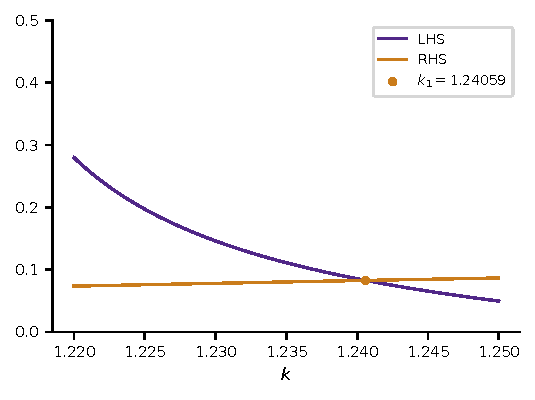
\includegraphics[width=\linewidth,height=.36\textheight,keepaspectratio]{figures/drafts/lesson38_cell46.pdf}
\end{center}
% End notebook cell 46

% Notebook cell 47 (markdown)
\Needspace{12\baselineskip}
The actual reactivity worth is, therefore,

\[
  \delta \rho = \frac{k_1-k_0}{k_1 k_0} \approx -0.01079 \, ,
\]

which is even \emph{smaller} than the first-order perturbation theory estimate of \(\rho_{pt} = -0.01647\) and naïve estimate of \(\rho_{np} = -0.02041\).

So, to conclude, first-order perturbation theory gives us a better estimate than the naïve approach for about the same amount of work, and for much less work than the direct perturbation result.

One might have hoped for a ``better'' estimate, but consider again our perturbation, which was a 10\% increase in \(\Sigma_a\) in one third of the core. That may seem small, but it has a profound impact on the flux, which went from a pure cosine to a mixed shape involving several functions.
% End notebook cell 47

% Notebook cell 48 (markdown)
As a final step, let's plot the original and perturbed fluxes. For the perturbed flux, we still need \(C_3\), which we can get using flux continuity:
% End notebook cell 48

% Notebook cell 49 (code)
\begin{NEunicodecode}
cc_flux = sy.Eq(phi_I_sub.subs(x, a/6), phi_II_sub.subs(x, a/6))
coef3 = sy.solve(cc_flux, C3)[0]
phi_I_num = sy.lambdify(x, phi_I_sub.subs(buckling).subs(num_data).subs(k, k_1))
phi_II_num = sy.lambdify(x, phi_II_sub.subs(C3, coef3).subs(buckling).subs(num_data).subs(k, k_1))
\end{NEunicodecode}
% End notebook cell 49

% Notebook cell 50 (code)
\begin{NEunicodecode}
x_full = np.linspace(-25, 25, 2000)
plt.plot(x_full, np.cos(B_0*x_full), 'k')

x_I = np.linspace(-25, 50/6, 1000)
x_II = np.linspace(50/6, 25, 1000)
plt.plot(x_I, phi_I_num(x_I), 'b')
plt.plot(x_II, phi_II_num(x_II), 'b--')

plt.legend(['unperturbed', 'perturbed'])
plt.xlabel("$x$ [cm]")
plt.ylabel("$\phi(x)$ [cm]");
\end{NEunicodecode}
% Stored notebook output 0 (image/png).
\begin{center}
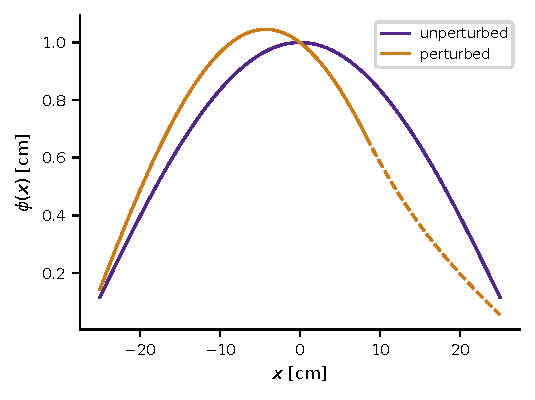
\includegraphics[width=\linewidth,height=.36\textheight,keepaspectratio]{figures/drafts/lesson38_cell50.pdf}
\end{center}
% End notebook cell 50

\end{handoutflow}
\end{document}
